\chapter{State of the art}

\section{Current state of networks solution}

Starting from the Introduction's consideration, I'm going to list the details of the three main solutions for 
blockchain networks\cite{private-public}:

\begin{outline}
    \1 \textbf{Public blockchains}: they are peer to peer networks in which anyone in the world has read 
    access to the network, anyone can send transactions over the network, and anyone in the world can 
    participate in the consensus process. In a public blockchain every node is potentially 
    untrusted, so the consensus mechanism is developed in order to prevent every malicious node that could 
    compromise data and transactions performed over the network. The entire architecture and consensus are 
    distributed in order to minimize the liability of data manipulation. The consensus process defines the blocks that get added to the chain
    determining the current state of the network. The security issue is solved by a mix of cryptographic algorithms
    and cryptoeconomics solution. The idea is to combine economic incentives proportional to the resources that
    the node can bring to bear. The resources targeted depend on the consensus algorithm used. For example proof of work(PoW)
    involves computational resources into the consensus mechanism. On the other hand, proof of stake(PoS) involve
    the token amount of the node involved in consensus. These blockchains are generally considered 
    to be "fully decentralized".
    \1 \textbf{Consortium blockchains}: The basic idea of the consortium blockchain is that the network is 
    composed by a set of trusted or semi-trusted nodes, that compose the governance of the network.
    The consensus mechanism is not as complex as that of public blockchains, because the starting hypothesis is 
    different and usually it needs to have a good performance and low latency of the transactions.
    I provide an example to understand how governance's nodes are involved in the consensus process: 
    One might imagine a consortium of 15 financial institutions, each of them operates a node and 10 of them 
    must sign every block in order for the block to be valid. The right to read the blockchain may be public, 
    or restricted to the participants, and there are also hybrid routes such as the root hashes of the blocks 
    being public together with an API that allows members of the public to make a limited number of queries 
    and get back cryptographic proofs of some parts of the blockchain state. These blockchains may be 
    considered "partially decentralized".
    \1 \textbf{Fully private blockchains}: a fully private blockchain is a blockchain where write permissions 
    are kept centralized to one organization. Read permissions may be public or restricted to an arbitrary 
    extent. Likely applications include database management, auditing, etc internal to a single company. Therefore, 
    public readability may not be necessary at all in many cases, although, in other cases public auditability 
    is desired.
\end{outline}

\subsection{Behind the Blockchains}
With the blockchain technology, cryptographic science found the most applications. The concept behind 
the public blockchain is that all the transaction data are completely public; nevertheless, the identity of the 
user involved is kept secret. This idea has found a huge application in the cryptocurrencies environment. 
The \textit{Fintech} is the environment in which the public blockchains has found the most applications. 
The main rule of the overall system is 
\textbf{"keep it transparent , safe and anonymous"}, it means that all the transactions processed by the 
public blockchain networks are \textbf{transparent } and every node has read access. The \textbf{Safe}
concept is granted by the combination of cryptographic science and economic incentives. \textbf{Anonymous}
has granted thanks to the cryptographic science applications, for example, the bitcoin wallet is based on a key pair 
computed on elliptic curve algorithms. If no one shares the identity associated with the wallet public key, or keep 
the private key public, the user identity continues to be anonymous. 
\bigskip


\bigskip
As explained above the blockchain world is divided between public and private blockchain.  
To understand the behavior about public or private blockchains, we are going to list the features
for both, in order to adapt the choice based on own needs: 

\begin{outline}[enumerate]
    \1 The main advantages of the \textbf{Public blockchain} could fall into two major categories:
    \2 Public blockchains provide a way to protect the users of an application from the developers; 
    the code is public and everyone can see how it works. This solution limits the authority 
    of the developers over the application. Moreover, the user identity is always kept secret .   
    \2 Public blockchains are open, and therefore are likely to be used by many entities and gain 
    some network effects. Besides, the public blockchain fully eliminates intermediaries. Here is an example 
    of a transfer of ownership case. A wants to sell an item to B. Right now there is a standard risk 
    problem of the involved counterparty: if A sends first, B may not send money, and if B sends first the 
    money A might not send the item. All the problems related to these kinds of cases could be resolved using 
    smart contracts, running over the public blockchain, moreover, the costs is close to zero. 
    With the smart contract implementations, A can send the item, to be sold, to a program that immediately 
    sends it to the first person that in the meanwhile sends money to the program. 
    
    \1 Compared to the public blockchain, the advantages of a \textbf{Private blockchain} are:

    \2 The consortium or companies running a private blockchain can easily, if desired, change the rules 
    of a blockchain, revert transactions, modify balances, etc. In some cases, eg. national land 
    registries, this functionality is necessary.
    
    \2 The validators are known, so any risk of a 51\% attack, arising from some miner collusion in China, 
    does not apply.

    \2 Transactions are cheaper, since they only need to be verified by a few nodes that can be trusted 
    to have very high processing power, and do not need to be verified by ten thousand laptops. This is 
    a hugely important concern right now, as public blockchains tend to have transaction fees exceeding 
    \$0.01 per tx.

    \2 Nodes can be trusted to be very well-connected, and faults can quickly be fixed by manual intervention, 
    allowing the use of consensus algorithms which offer finality after much shorter block times. 

    \2 If read permissions are restricted, private blockchains can provide a greater level of, well, privacy.
\end{outline}

From many analysis it gets out that the 75\% of already implemented projects are designed specifically for 
private aim \cite{blockchain-state},
which means that a need is growing to improve the Consortium Blockchains that allow a memberships 
mechanism build for company use cases, which maintains the transactions private to guarantee the privacy of 
the business process and data.
\\
On the other hand, in some processes it is useful to implements public blockchain solutions, so there is a growing need to 
improve the interoperability about a consortium and public blockchains into a cross-chain solution.

%{\renewcommand{\arraystretch}{2}%
%\begin{tabular}{|l|l|l|l|l|}
%  \hline
%  \textbf{Blockchain Name} & \textbf{Network} & \textbf{Currency} & \textbf{Consensus} & \textbf{Smart Contract} \\
%  \hline
%  \textbf{Bitcoin} & Public & Bitcoin & PoW & Possible but less extendible\\
%  \hline
%  \textbf{Ethereum} & Public & Ether & PoS & Multiple programming languages\\
%   ~ & ~ & ~ & ~ & (Solidity, Vyper)\\
%   \hline
%   \textbf{Hyperledger} & Permissioned - & None & Pluggable or & Multiple programming languages\\
%  ~ & Federal/Private & ~ & PBFT & (Go, Java, Javascript, Solidity)\\ 
%  \hline
  %\textbf{Eos} & No & Yes & Yes\\
  %\hline 
  %\label{table:compare-blockchains}
%\end{tabular}}

%\begin{table}[htbp]
%    \centering
%    \begin{tabular}{|c|c|c|c|c|p{1cm}p{1cm}p{1cm}p{1cm}p{1cm}p{1cm}p{1cm}|}
%    \hline
%    \textbf{Blockchain Name} & \textbf{Network} & \textbf{Currency} & \textbf{Consensus} & \textbf{Smart Contract}  \\ \hline
%    \textbf{Bitcoin} & Public & Bitcoin & PoW & Possible but less extendible \hline
%    \multirow{ 2}{*}{1} \textbf{Ethereum} & Public & Ether & PoS & Multiple programming languages \\
%    ~ & ~ & ~ & ~ & (Solidity, Vyper)\hline
%    \multirow{ 2}{*}{1} \textbf{Hyperledger} & Permissioned - & None & Pluggable or & Multiple programming languages \\
%    ~ & Federal/Private & ~ & PBFT & (Go, Java, Javascript, Solidity)\hline
%    \end{tabular}
%    \caption{A test caption}
%    \label{table1}
%\end{table}

\begin{table}[h]
    {\renewcommand\arraystretch{1.25}
    \begin{tabular}{|l|l|l|l|l|} \hline
    \textbf{Name} & \textbf{Network} & \textbf{Currency} & \textbf{Consensus} & \textbf{Smart Contract}\\ \hline\hline
    \textbf{Bitcoin} & Public & Bitcoin & PoW & Possible but less extendible\\ \hline
    \textbf{Ethereum} & Public & Ether & PoS & Solidity, Vyper\\ \hline
    \textbf{Hyperledger} & Permissioned & None & PBFT & Go, Java, Javascript, Solidity\\ \hline
    \end{tabular}}
    \caption{Comparing among blockchains features}
    \label{table-compare-blockchains}
\end{table}

\subsection{Overview}

Michael Burgess, chief operating officer of Ren states that \textbf{"All interoperability solutions will 
likely have trade-offs; so it's a matter of designing systems that find a balance between security, 
governance, adaptability, and economic incentives that suit their target market."}
\bigskip

\textbf{"Private chains operating without distributed consensus are more prone to data manipulation 
and the integrity of the data/assets being transferred from a private, permissioned and centralized 
chain to a more decentralized chain could be questioned. Overall, there is no one solution that fits 
all in terms of being public/private, centralized/decentralized — it is a broad spectrum with specific 
trade-offs."}\cite{interoperability1}
, quoting the words of Agarwal, CEO of Persistence.
\bigskip

What is getting from the point of view of the industry experts; it is a trade-off solution to obtain cross-chain 
interoperability, between public and private.

\subsection{Limitations}

Considering the pros and cons of each network listed, interoperability could in some cases be the 
solution of many cases problem, for example, the public blockchain could allow an asset transaction among 
users without limit and granted security and authentication. On the other hand, consortium solution could 
allow companies to set up roles over their own network and to keep information data private. Nevertheless, 
the integration between the two blockchain solutions has several Achilles heels to be evaluated and managed:


\begin{outline}
    \1 \textbf{Synchronization}: both networks must be synchronized and the world state must be the same in 
    each moment. This means that each transaction that involves both blockchains, must reach strong synch among 
    the ledgers, before being archived

    \1 \textbf{Time Effort}: in order for it to be usable, the transactions and synchronization
    must be performed in a reasonable time.
    
    \1 \textbf{Identity}: each blockchain implementation handles the identity mechanism in a specific way. 
    This means that the user wallet is implemented using specific cryptographic algorithms and solutions. For 
    example, Ethereum handles it as a Key pair, private and public, that allow authentication of the wallet 
    owner, on the other hand, Hyperledger Fabric implements the authentication mechanism for the user of the 
    network using x.509 certificates. So the other problem is the mapping of these different mechanisms that 
    blockchains implement to allow authentications. 
\end{outline}


\subsection{CrossChain Current Solution}

The new challenge of cross-chain was born a few years ago and it has brought many companies and research centers 
to design solutions to fix the problem and allow interoperability. The \textbf{Figure \ref{fig:crosschain-interaction}} 
shows the theoretical solution to the interoperability problem between Bitcoin and Ethereum, at each layer of 
blockchain architecture\cite{crosschain-level}.

\begin{figure}[h!]
	\centering
	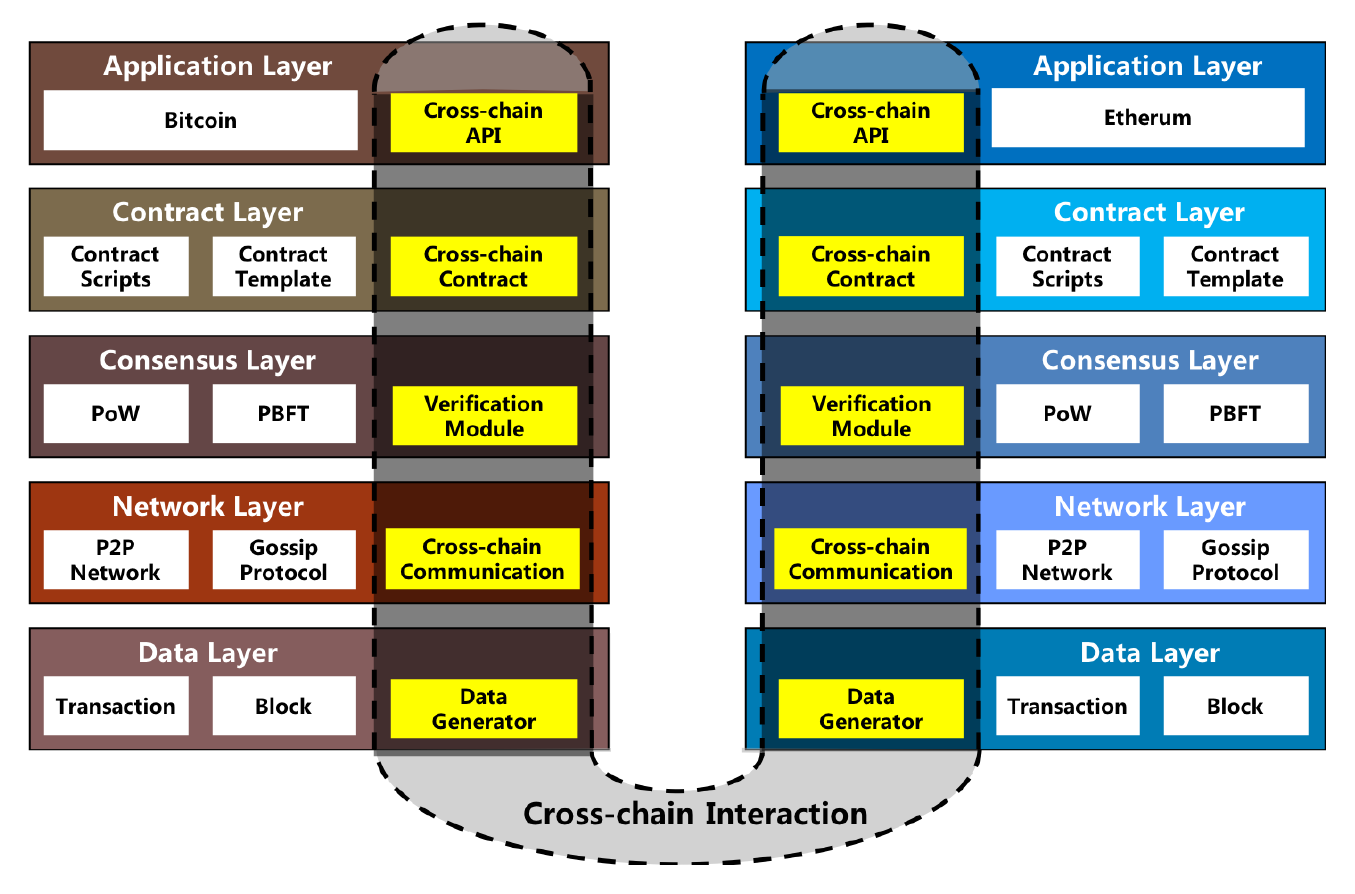
\includegraphics[totalheight=6cm]{img/crosschain.PNG}
	\caption{CrossChain Interactions}
	\label{fig:crosschain-interaction}
\end{figure}

The main ideas to perform interoperability is:

\begin{outline}
    \1 \textbf{New Blockchain}: Over the last few years several networks and frameworks have appeared that propose to 
    allow the interconnection between public and private blockchains. Many of those solutions are based on new 
    blockchain networks that are structured in order to allow, architectural level, the interoperability, for 
    example, Ark\cite{ark} is a blockchain-based platform that allows anyone to customize their own blockchain. But 
    the biggest challenges still remains to allow interconnection between the well-known blockchain 
    networks. 

    \1 \textbf{Architectural Framework}: There are thousands of frameworks proposed over the last few years, but 
    the cross-chain isn't still a consolidated reality. Nevertheless, most of the solutions share the same idea, a 
    Sidechain\cite{sidechain} between the two blockchains. Introducing a new layer between the two mainnet that allows 
    mapping, using ad-hoc API, the requests from one network to the other one. In a nutshell all the requests 
    from the one to the other blockchain and vice-versa passing by the sidechain.\cite{atomic-crosschain} \cite{iot-crosschain}

    \1 \textbf{Atomic Swaps}\cite{atomic-swap}: it allows users to trade one cryptocurrencies for another directly in a peer-to-peer 
    transaction Hashed TimeLock Contracts (HTLCs)\cite{HTLC}. Atomic swaps are not a true form of cross-chain 
    communication (as the two chains do not communicate), but a mechanism that allows two parties to 
    coordinate transactions across chains. Atomic swaps can be effective if used correctly and are they are the 
    mechanism that enables the Lightning Network\cite{lightning}.

    \1 \textbf{Relay}: it allows a contract to verify block headers and events on another chain. Several 
    approaches to relays exist, ranging from verifying the entire history of a chain to verifying specific 
    headers on-demand. Each method has trade-offs between the cost of operation and the security of the relay. 
    Relays are often quite expensive to operate, as we saw first-hand with BTCRelay\cite{relay}.

    \1 \textbf{Merged Consensus}: it allows for two-way interoperability between chains through the use of a relay 
    chain. Merged consensus can be quite powerful, but generally must be built into the chain from the ground 
    up. Projects like Cosmos\cite{cosmos} and ETH2.0\cite{eth2} 
    use merged consensus.

    \1 \textbf{Federations}: it allows a selected group of trusted parties to confirm the events of one chain on 
    another. While federations are powerful, their obvious limitation lies in the requirement to trust a 
    third party.

\end{outline}

\subsection{Chaincode EVM}

In the thesis work, I focused my attention on Hyperledger and Ethereum, two of the main blockchain 
solutions used in the world, the former for permissioned cases, the latter one for public processes. 
In the last year, IBM technical ambassador developed an \textbf{EVM chaincode}\cite{evm-chaincode} 
able to run bytecode of Solidity smart contract over the Hyperledger Fabric network. It is not a real 
cross-chain solution but it is a step forward interoperability among blockchains. It still has many limits, 
for example, there isn't a real identity mapping mechanism from eth address to fabric identity and vice-versa. 

\section{Blockchain application in Fashion Environment}

\subsection{Provenance case & Martine Jarlgaard}

Thanks to the blockchain feature it is possible to store in an immutable way the record associated with each 
transaction performed over the supply chain.  One of the first fashion houses that started to use the blockchain 
technology for its own company is Martine Jarlgaard that in 2017, the fashion company made a partnership with Provenance\cite{provenance} 
producing clothes with digital tag: The tag could be a QRCode od an RFID reader using NFC technology.
That tag provides the entire history of the related clothes, providing each step of the producing process.
\bigskip

The actors of the supply chain process are:

\begin{outline}
    \1 \textbf{British Alpaca Fashion Farm}: It cares about alpacas livestock and shearing.
    \1 \textbf{Two Rivers Mill}: It cares about wool spinning.
    \1 \textbf{Knitster LDN}: It cares about the knitting process.
    \1 \textbf{Martine Jarlgaard}: It cares about the design of the clothes and the final work.
\end{outline}

Each actor of the supply chain is a blockchain node that takes part in the supply chain pipe through 
the transactions of the exchanged assets, such as wool, cloth, and so on. Each transaction is registered over the 
blockchain and visible at each node. 

Customer side the user has a clear vision of the entire production process, from the material used to the 
item produced. It allows the company to gain credibility and transparency of the products sale. 

\subsection{Counterfeiting - VeChain & BabyGhoast}

BabyGhoast by combining blockchain technology with NFC chips, it creates a digital identity for each cloth 
produced. It improved the tracking process over the supply chain. Moreover, it allows protecting the brand 
and the users against counterfeit items. In order to implement the solution it is used VeChain technology, that includes 
inside BabyGhoast clothes an RFID/NFC chip or QRCode, that allows identification of the item thanks to a 
unique ID VeChain. Moreover, by scanning the chip or QRCode using the VeChain Pro application, it is possible to 
access the data related to the item and the production process. 

\section{Use Case asis}

Armadio Verde is an Italian community that was born to share children's clothes. Once it grew up, it allows 
adult clothes sharing too. The working model is based on the sharing principle. Every user, after is signing up 
to the platform, can book a pick up of their old clothes. The clothes must be in a good state, clean and 
put in a box. Once the box arrives at Armadio Verde, the clothes are going to be checked and evaluated. For each 
approved clothes, a dedicated form  is created with all the related information. After the upcycling process, 
the clothes are shared over the platform store. The user that sent the clothes earns an amount of 
"star"(the money used over the platform). The star could be used to purchase other clothes adding a few euros 
for each item. The clothes that could not be shared on the platform for the reselling process, are sent to a 
certified Onlus.

\subsection{Sustainability Token}

\subsubsection{PlasticToken}

Plastic Token is an ERC20 chaincode that runs over the Hyperledger Fabric network\cite{plastic-coin}. It provides functionalities to read
and write, with access and rights control, into the distributed ledger. The ERC20 chaincode is the software 
securely handling the PlasticTokens. These tokens are up to the ERC20 standard, meaning a fixed 
amount of tokens will be minted when the chaincode is deployed. This amount is called “TotalSupply” and 
will be assigned to a special user, called “central bank” in the current implementation.
Once the original PlasticToken\cite{ptwist} supply is minted, users can interact with it via a “transfer” functionality. It
allows the central bank to send tokens to any previously enrolled user, then each user can use this same
function to transfer tokens between each other

It runs over the Plastic Twist project. 

\subsubsection{ECOCoin}

The ECO coin\cite{eco-coin} is a new cryptocurrency that is earned through sustainable action. The ECO coin
aims to reward anyone, anywhere in the world carrying out sustainable actions. Eating meat-free
meals, switching to a green energy provider or riding a bike to work can earn you ECOs which
users could spend in ECO new sustainable marketplace to buy ecological experiences, services and
goods. 

It is based on consortium blockchain architecture and each marketplace that want to involve their 
business in ECO environment must be accepted as a governance member of the network. 